\documentclass[12pt,a4paper]{article}
\usepackage[utf8]{inputenc} %polskie znaki
\usepackage[T1]{fontenc}	%polskie znaki
\usepackage{amsmath}		%matematyczne znaczki :3
\usepackage{enumerate}		%Dodatkowe opcje do funkcji enumerate
\usepackage{geometry} 		%Ustawianie marginesow
\usepackage{graphicx}		%Grafika
\usepackage{wrapfig}		%Grafika obok textu
\usepackage{float}			%Allows H in fugire
%\pagestyle{empty} 			%usuwa nr strony

\newgeometry{tmargin=2cm, bmargin=2cm, lmargin=2cm, rmargin=2cm} 

\begin{document}
	\begin{center}
		\LARGE Kombinatoryka i Rachunek Prawdopodobieństwa
	\end{center}
	\vspace{1cm}
	\begin{enumerate}[1.]
	\item Na ile sposobów można rzucić dwa razy kostką sześcienną?
	\item Na ile sposobów możemy wrzucić pięć kul do sześciu różnych szuflad?
	\item Ile różnych liczb trzycyfrowych można utworzyć z cyfr $\{1,2,3,\dots,9\}$?
	\item Ile różnych liczb pięciocyfrowych można utworzyć z cyfr $\{0,1,2,3,4,5\}$?
		\item Ile jest liczb trzycyfrowych, w których:
	\begin{enumerate}[a)]
		\item występują tylko cyfry nieparzyste?
		\item występują tylko cyfry parzyste?
		\item co najmniej jedna cyfra jest parzysta?
		\item co najmniej jedna cyfra jest nieparzysta?
		\item pierwsza i ostatnia cyfra jest taka sama, a druga jest równa 5 albo 8?
		\item 7 występuje dokładnie jeden raz, a ostatnia cyfra jest podzielna przez 3?
	\end{enumerate}
	\item Do windy wsiada 5 osób, które mogą wysiąść na 10 różnych piętrach. Na ile sposobów mogą:
	\begin{enumerate}[a)]
		\item wysiąść dowolnie?
		\item wysiąść tylko na 3, 5 lub 7 piętrze?
		\item wysiąść na różnych piętrach?
		\item wysiąść tak, aby przynajmniej jedna osoba wysiadła na 7 piętrze?
	\end{enumerate}
	\item Każdej z 10 osób przyporządkowujemy miesiąc, w którym się urodził. Ile jest możliwych przypadków, że:
	\begin{enumerate}[a)]
		\item każda osoba urodzi się innego miesiąca?
		\item wszystkie osoby urodzą sie tego samego miesiąca?
		\item żadna osoba nie urodziła się ani w styczniu, ani w grudniu?
	\end{enumerate}
\newpage
	\item W autobusie, który ma przed sobą 10 przystanków siedzi 7 osób. Zakładając, że do autobusu nie wsiądą żadne nowe osoby, na ile sposobów osoby te mogą wysiąść:
	\begin{enumerate}[a)]
		\item na dowolny sposób?
		\item tak aby każda osoba wysiadła na innym przystanku?
	\end{enumerate}
	\item Ile jest różnych kodów PIN, w których cyfry a) mogą / b) nie mogą się powtarzać?
	\item Pani Barbara ma w szafie czapkę zieloną, białą i czarną, szal zielony i czarny oraz rękawiczki niebieskie, białe, czarne i różowe. Na ile sposobów Pani Barbara może:
	\begin{enumerate}[a)]
		\item różnie się ubrać?
		\item wyrać zestaw tego samego koloru?
		\item wybrać zestaw, który zawiera przynajmniej dwa takie same kolory?
	\end{enumerate}
	\item Ile jest telefonicznych numerów komórkowych, składających się z dziewieciu cyfr takich, że:
	\begin{enumerate}[a)]
		\item pierwszą cyfrą jest 5 lub 6, trzecią cyfrą jest 0, a pozostałe nie są ani piątką, ani szóstką?
		\item każda cyfra jest inna i na pierwszym miejscu nie występuje 0?
		\item każda kolejna cyfra tego numeru jest liczbą o 1 mniejszą od poprzedniej?
		\item podane cyfry tworzą ciąg malejący?
		\item pierwsza, trzecia, piąta i siódma cyfra jest taka sama i jest nieparzysta, zaś pozostałe są liczbami parzystymi?
	\end{enumerate}
	\item Mamy 5 książek, w tym książki A i B. Ustawiamy je losowo na pustej półce, jedna obok drugiej. Na ile sposobów można ustawić je tak, aby:
	\begin{enumerate}[a)]
		\item książki A i B stały obok siebie?
		\item pomiędzy książkami A i B stały dokładnie dwie inne książki?
		\item książki książka A była na lewo od książki B?
	\end{enumerate}
\item Z grupy 5 kobiet i 4 mężczyzn wybieramy dwie osoby. Ile jest takich sposobów wyboru tej delegacji tak, aby wśród wybranych osób:
\begin{enumerate}[a)]
	\item były same kobiety?
	\item była kobieta i mężczyzna?
\end{enumerate}
\item W klasie jest 15 dziewcząt i 16 chłopców. Spośród uczniów tej klasy wybieramy losowo trzech przedstawicieli do konkursu. Na ile sposobów można wybrać tą delegację tak aby:
\begin{enumerate}[a)]
	\item wybrać tą delegację?
	\item był tam dokładnie jeden chłopak?
	\item były tam co najmniej dwie dziewczynki?
	\item były tam co najwyżej dwie dziewczynki?
\end{enumerate}
\newpage
\item W urnie jest 7 kul białych, 2 czarne i 1 zielona. Ile jest możliwych sposobów wyboru dwóch kul z tej urny tak, aby:
\begin{enumerate}[a)]
	\item kule były różnych kolorów?
	\item obie kule były białe?
	\item obie kule były tego samego koloru?
	\item przynajmniej jedna z kul była biała?
\end{enumerate}
\item W urnie jest 5 kul białych, 4 czarne i 7 zielonych. Losujemy trzy kule. Ile jest możliwych wyników losowania tak, aby:
\begin{enumerate}[a)]
	\item każda z wylosowanych kul była innego koloru?
	\item wszystkie trzy kule mają być tego samego koloru?
	\item wśród trzech kuli dwie muszą być tego samego koloru?
\end{enumerate}
\item Ile różnych wyrazów (mających sens lub nie) można ułożyć z wyrazów:
\begin{enumerate}[a)]
	\item STRAJK
	\item KAJAK
	\item KANAPKA
	\item MATEMATYKA
	\item KONSTANTYNOPOLITAŃCZYKÓWIANECZKA*
\end{enumerate}
(* tam są 32 litery)
\item Z talii kart (52 kart) losujemy cztery karty. Na ile sposobów można wybrać karty:
\begin{enumerate}[a)]
	\item dowolnie?
	\item tak, aby były dwie damy i dwa asy?
	\item tak, aby były trzy karty "młodsze" od dziewiątki i jeden król?
	\item trzy figury i jedna karta nie będąca figurą?
	\item dwa kiery i pik?
	\item co najwyżej dwa trafle?
	\item kier i karo?
\end{enumerate}
\newpage
\item Rzucamy trzykrotnie symetryczną monetą, oblicz prawdopodobieństwo, że:
\begin{enumerate}[a)]
	\item wypadnie trzy razy orzeł.
	\item wypadnie reszka dokładnie dwa razy.
	\item orzeł wypadnie przynajmniej jeden raz.
\end{enumerate}
\item Rzucamy dwukrotnie sześcienną kostką do gry. Oblicz prawdopodobieństwo, że:
\begin{enumerate}[a)]
	\item wypadną dwie szóstki.
	\item nie wypadnie żadna szóstka.
	\item wypadnie przynajmniej jedna szóstka.
	\item liczba oczek będzie parzysta.
	\item suma oczek będzie większa niż 9.
\end{enumerate}
\item W talii 52 kart losujemy jedną kartę. Oblicz prawdopodobieństwo, że wylosowana karta:
\begin{enumerate}[a)]
	\item jest treflem lub pikiem.
	\item asem i nie jest treflem.
	\item królem lub kierem.
	\item kartą młodszą od siódemki.
\end{enumerate}
\item Ze zbioru liczb dwucyfrowych losujemy jedną liczbę. Oblicz prawdopodobieństwo, że wylosowana liczba jest:
\begin{enumerate}[a)]
	\item liczby podzielnej przez 2 lub 3.
	\item liczby podzielnej przez 5 i niepodzielnej przez 3.
\end{enumerate}
\item Oblicz prawdopodobieństwo wygrania w totka.
\item  Ze zbioru cyfr $\{1,2,3,4,5,6,7\}$ losujemy kolejno bez zwracania 2 cyfry i zapisujemy je wkolejnosci losowań, otrzymując liczbę dwucyfrowa. Oblicz prawdopodobieństwo, że będzie to liczba parzysta.
\item Do windy wsiadło 5 osób, które mogą wysiąść na 6 piętrach. Oblicz prawdopodobieństwo, że:
\begin{enumerate}[a)]
	\item wszystkie osoby wysiądą na jednym piętrze.
	\item każda osoba wysiądzie na innym piętrze.
\end{enumerate}
\item Rzucamy trzema sześciennymi symetrycznymi kostkami do gry. Oblicz prawdopodobieństwo, że suma otrzymanych oczek jest liczbą podzielną przez 8 i jednocześnie niepodzielną przez 16.
\item Rzucamy trzema czworościennymi symetrycznymi kostkami do gry (z oczkami 1,2,3,4). Oblicz prawdopodobieństwo, że suma otrzymanych oczek jest liczbą podzielną przez 3.
\item W pudełku znajdują się 4 losy wygrywające i 6 losów przegrywających. Losujemy kolejno bez zwracania po jednym losie. Oblicz prawdopodobieństwo wylosowania:
\begin{enumerate}[a)]
	\item dwóch losów wygrywających.
	\item przynajmniej jednego losu wygrywającego.
\end{enumerate}

	\item W urnie jest 20 kul ponumerowanych od 1 do 20. Wyjmujemy losowo jedną kulę. Oblicz prawdopodobieństwo, że numer na wylosowanej kuli będzie:
	\begin{enumerate}[a)]
		\item większy od 8
		\item podzielny przez 5
		\item liczbą pierwszą
	\end{enumerate}
	\item W pierwszej urnie są 2 kule białe i 4 kule czarne. W drugiej jest 1 kula biała i 4 kule czarne. Z każdej urny wyciągamy po jednej kuli. Oblicz prawdopodobieństwo, że wylosowane kule będą tego samego koloru.
	\item Oblicz prawdopodobieństwo, że w trzech rzutach symetryczną kostką sześcienną do gry suma kwadratów liczb uzyskanych oczek będzie podzielna przez 3.
	\item W pierwszej urnie są 3 kule białe, 2 czarne i 4 zielone. W drugiej urnie są 4 białe, 5 czarnych i 1 zielona. Losowanie polega na rzuceniu symetryczną monetą i jeśli wypadnie orzeł to losujemy z pierwszej urny, jeśli reszka to z drugiej urny. Oblicz prawdopodobieństwo wylowania kuli
	\begin{enumerate}[a)]
		\item białej
		\item czarnej
		\item zielonej
	\end{enumerate}
	
	\item Na sali jest 12 ławek w 4 rzędach. 12 uczniów losuje miejsca na sali. Jakie jest prawdopodobieńostwo, że studenci A, B i C będą siedzieli w tym samym rzędzie?
	
	\item Trzy osoby wsiadają losowo do pociągu, składającego się z 5 wagonów. Jakie jest prawdopodobieńostwo, że każda z tych osób odbędzie podróż w innym wagonie?
	
	\item Jakie jest prawdopodobieńostwo, że w losowo wybranej grupie 23 osób, znajdą się co najmniej dwie, które obchodzą urodziny tego samego dnia?
	
	\item W pudełku A znajduje się 5 kul białych i 7 kul czarnych. Wybieramy losowo jedną kulę. Jeżeli wylosujemy kulę białą losujemy ponownie jedną kulę z tego pudełka, a jeżeli wylosowaliśmy kulę czarną, losujemy jedną kulę z pudełka B, w którym znajduje się 7 kul białych i 8 kul czarnych. Jakie jest prawdopodobieńostwo, że w drugim losowaniu wybierzemy kulę białą?
	
	\item Dziecko bawi się literkami A, A, A, E, K, M, M, T, T, Y . Oblicz prawdopodobieństwo, że przypadkowo złoży
	ono słowo MATEMATYKA.
	
	\item W szafie jest 10 par butów. Losujemy 4 buty. Oblicz prawdopodobieństwo, że wylosujemy co najmniej jedną parę.
	
	\item W urnie jest 6 kul białych, 3 kule czarne i pewna liczba kul niebieskich. Oblicz ile jest kul niebieskich, jeżeli prawdopodobieństwo wylosowania kuli białej z tej urny wynosi $\frac{1}{3}$. 
\end{enumerate}

\newpage

\begin{center}
	\LARGE Statystyka
\end{center}
\vspace{1cm}
\begin{enumerate}[1.]
	\item Oblicz medianę i średnią arytmetyczną liczb: $\{2,\:4,\:5,\:3,\:7,\:9,\:-2\}$
	\item Średnia arytmetyczna liczb: $\{x,\:3,\:1,\:4,\:1,\:5,\:1,\:4,\:1,\:5\}$ jest równa 3. Oblicz "x".
	\item Poniższa tabela przedstawia wyniki sprawdzianu klasy IV
	
	\begin{tabular}{|c|c|c|c|c|c|c|}
		\hline
		Ocena&1&2&3&4&5&6\\
		\hline
		Liczba uczniów&2&4&5&6&2&1\\
		\hline
	\end{tabular}
	
	Oblicz medianę, średnią arytmetyczną i dominantę tych ocen.
	
	\item Średnia wieku w pewnej grupie studentów jest równa 23 lata. Średnia wieku tych studentów i ich opiekuna jest równa 24 lata. Opiekun ma 39 lat. Oblicz, ilu studentów jest w tej grupie.
	
	\item Przeprowadzono badania, dotyczżce liczby osób jadżcych w samochodach osobowych w godzinach rannych, w kierunku centrum pewnego miasta. Wyniki badań przedstawione są na digramie kołowym.
	
	\begin{figure}[h]
		\centering
		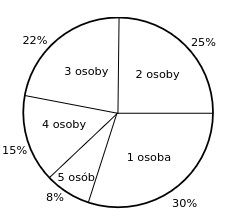
\includegraphics{stat1.jpeg}
	\end{figure}
	\begin{enumerate}[a)]
		\item Oblicz śrędnią liczbę osób jadących w samochodzie osobowym w godzinach rannych. Wyznacz również medianę i dominantę.
		\item Oblicz prawdopodobieństwo, że w losowo wybranym samochodzie osobowym, w godzinach
		rannych, w kierunku centrum, były więcej niż 3 osoby.
		\item Wiedząc, że samochodów osobowych, w których były 4 osoby, zaobserwowano o 350 więcej,	niż samochodów w których było 5 osób, oblicz, ile wszystkich samochodów obserwowano w
		trakcie badań.
	\end{enumerate}
\end{enumerate}
\end{document}